\section{Method}
\label{sec:model}

In this section we describe our approach Deep Cascade Multi-task Learning in detail.
\figref{fig:model}(d)(e) gives an overview of the proposed architecture.

\begin{figure*}[h]
	\centering
	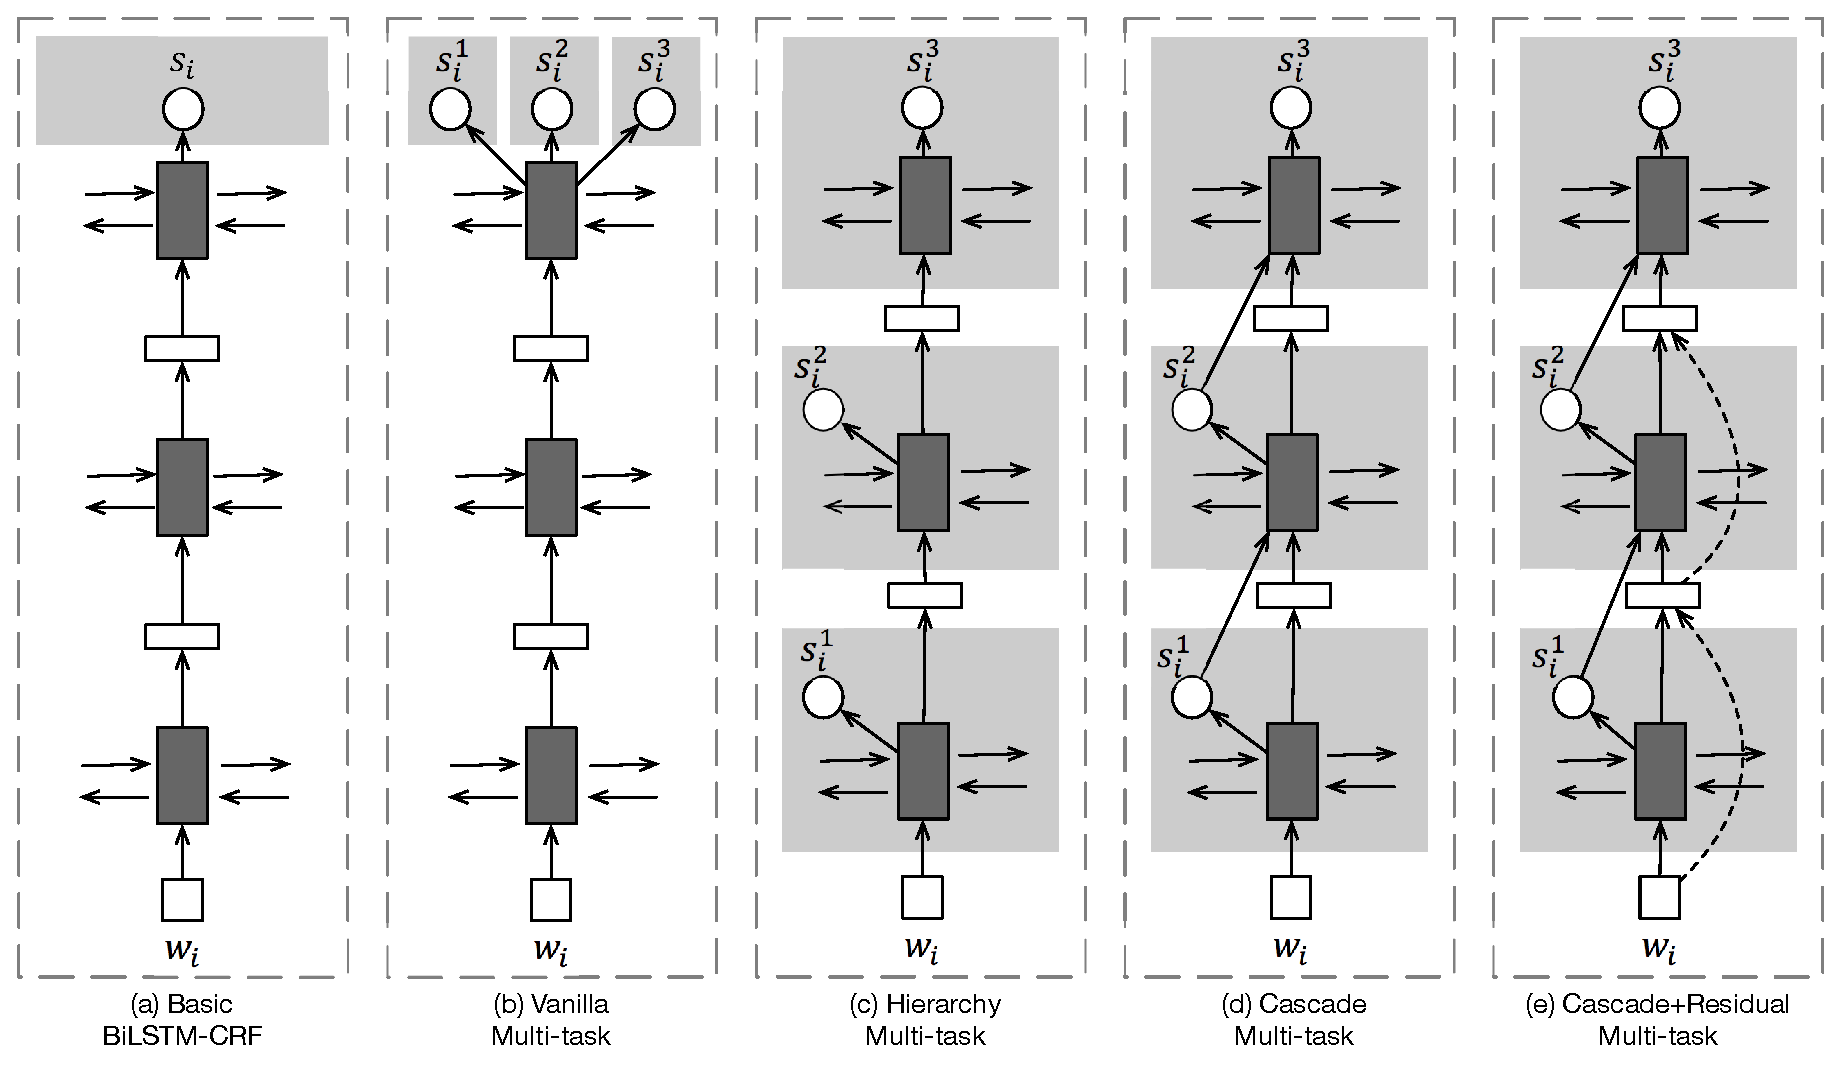
\epsfig{file=figures/model.eps, width=1.8\columnwidth}
	\caption{}
	\label{fig:model}
	\vspace{-10pt}
\end{figure*}

\subsection{Multi-task Learning}
\yu{Why Multi-task Learning?}
You can follow \secref{sec:slot_filling} to see we have a large number of slot labels
to be assigned to each word in the input utterance.
However due to the limited training data,
%the problem of sparsity becomes more serious for the tagging performance.
if we end-2-end train the high-level slot filling task (can be seen as semantic labeling task),
some low-level tasks such as name entity tagging or segment tagging (can be seen as syntactic labeling task)
may make mistakes first for the sparsity problem.
If the low-level tasks get wrong, so as to the target slot filling task.
But training low-level tasks is much more easier,
so we claim that 

In a multi-task learning (MTL) setting, we have several prediction tasks over the same input space.
Each task has its own output vocabulary (a task specific labels set),
but all of them map the length $n$ input sequence into a length $n$ output sequence.
Intuitively, \yu{Why MTL works?}

\subsection{Deep Cascade Multi-task Learning}

\subsubsection{Cascade Connection}

\subsubsection{Residual Connection}

\subsubsection{Training}